\documentclass[10pt,letterpaper]{article}
\usepackage{amsmath,amssymb,geometry,graphicx}
\usepackage{enumitem}
%\settextfont{B Nazanin}
\usepackage{lipsum}
\setlength{\parskip}{3mm}
\setlength{\parindent}{0mm}
\newcommand{\wid}{0.49\textwidth}
\newcommand{\widone}{60mm}
\begin{document}
\Large
\begin{center}
In the name of beauty

11th problem set of ComNet course

\hrulefill
\end{center}
Q1) 
\begin{enumerate}[label=\alph*-]
\item
At which layer is SSL implemented and why?
\item
Why does sequence numbering prevent an intruder from re-ordering segments? What happens if the sequence numbers are not encrypted by hash (i.e. only the data and the MAC key are included in hash calculations)?
\item
For what reason, is network-layer security said to provide “blanket coverage” and what does this terminology mean?
\item
What is Security Policy Database (SPD) and what does it stand for?
\end{enumerate}

Q2) 
\begin{enumerate}[label=\alph*-]
\item
What problem can be caused when a duplicate key is used in WEP?
\item
Since MK is a shared key between the client and the authentication server, how can we generate a shared key between the client and the access point?
\item
Assume that an attacker wants to perform a DoS (Denial of Service) attack by sending TCP ACK segments to an internal network. A solution is to configure the internal firewall to block (i.e. drop) all the incoming TCP ACK segments. What problem does this solution make and how to bypass it?
\end{enumerate}

Q3) A specific 4-bit to 4-bit look-up table, converts 4-bit strings $x$ to $c(x)$ as $$c(x)=(x_{10}\cdot 13\mod 16)_2,$$meanwhile, the function first converts the 4-bit blocks of the plain text to decimal. Then, multiplies it in 13 and gives the binary representation of the remainder of its division by 16.

\begin{enumerate}[label=\alph*-]
\item
Prove that this function gives unique output cipher sequences (i.e. no two 4-bit inputs lead to a same output) by finding its mapping table (similar to Table 8.1 of the textbook).
\item
Use the following example for block cipher with plain text = 10101101 and 4-bit chunks of data (instead of 8-bit) to obtain the cipher text. Assume there are 2 rounds in a loop and the scrambler inverts the incoming bits (e.g. maps 10010111 to 11101001).
\item
(Extra Mark) What number, in general, can we place instead of 13 to preserve the uniqueness of the look-up table?
\end{enumerate}

\begin{figure}[htbp]
\centering
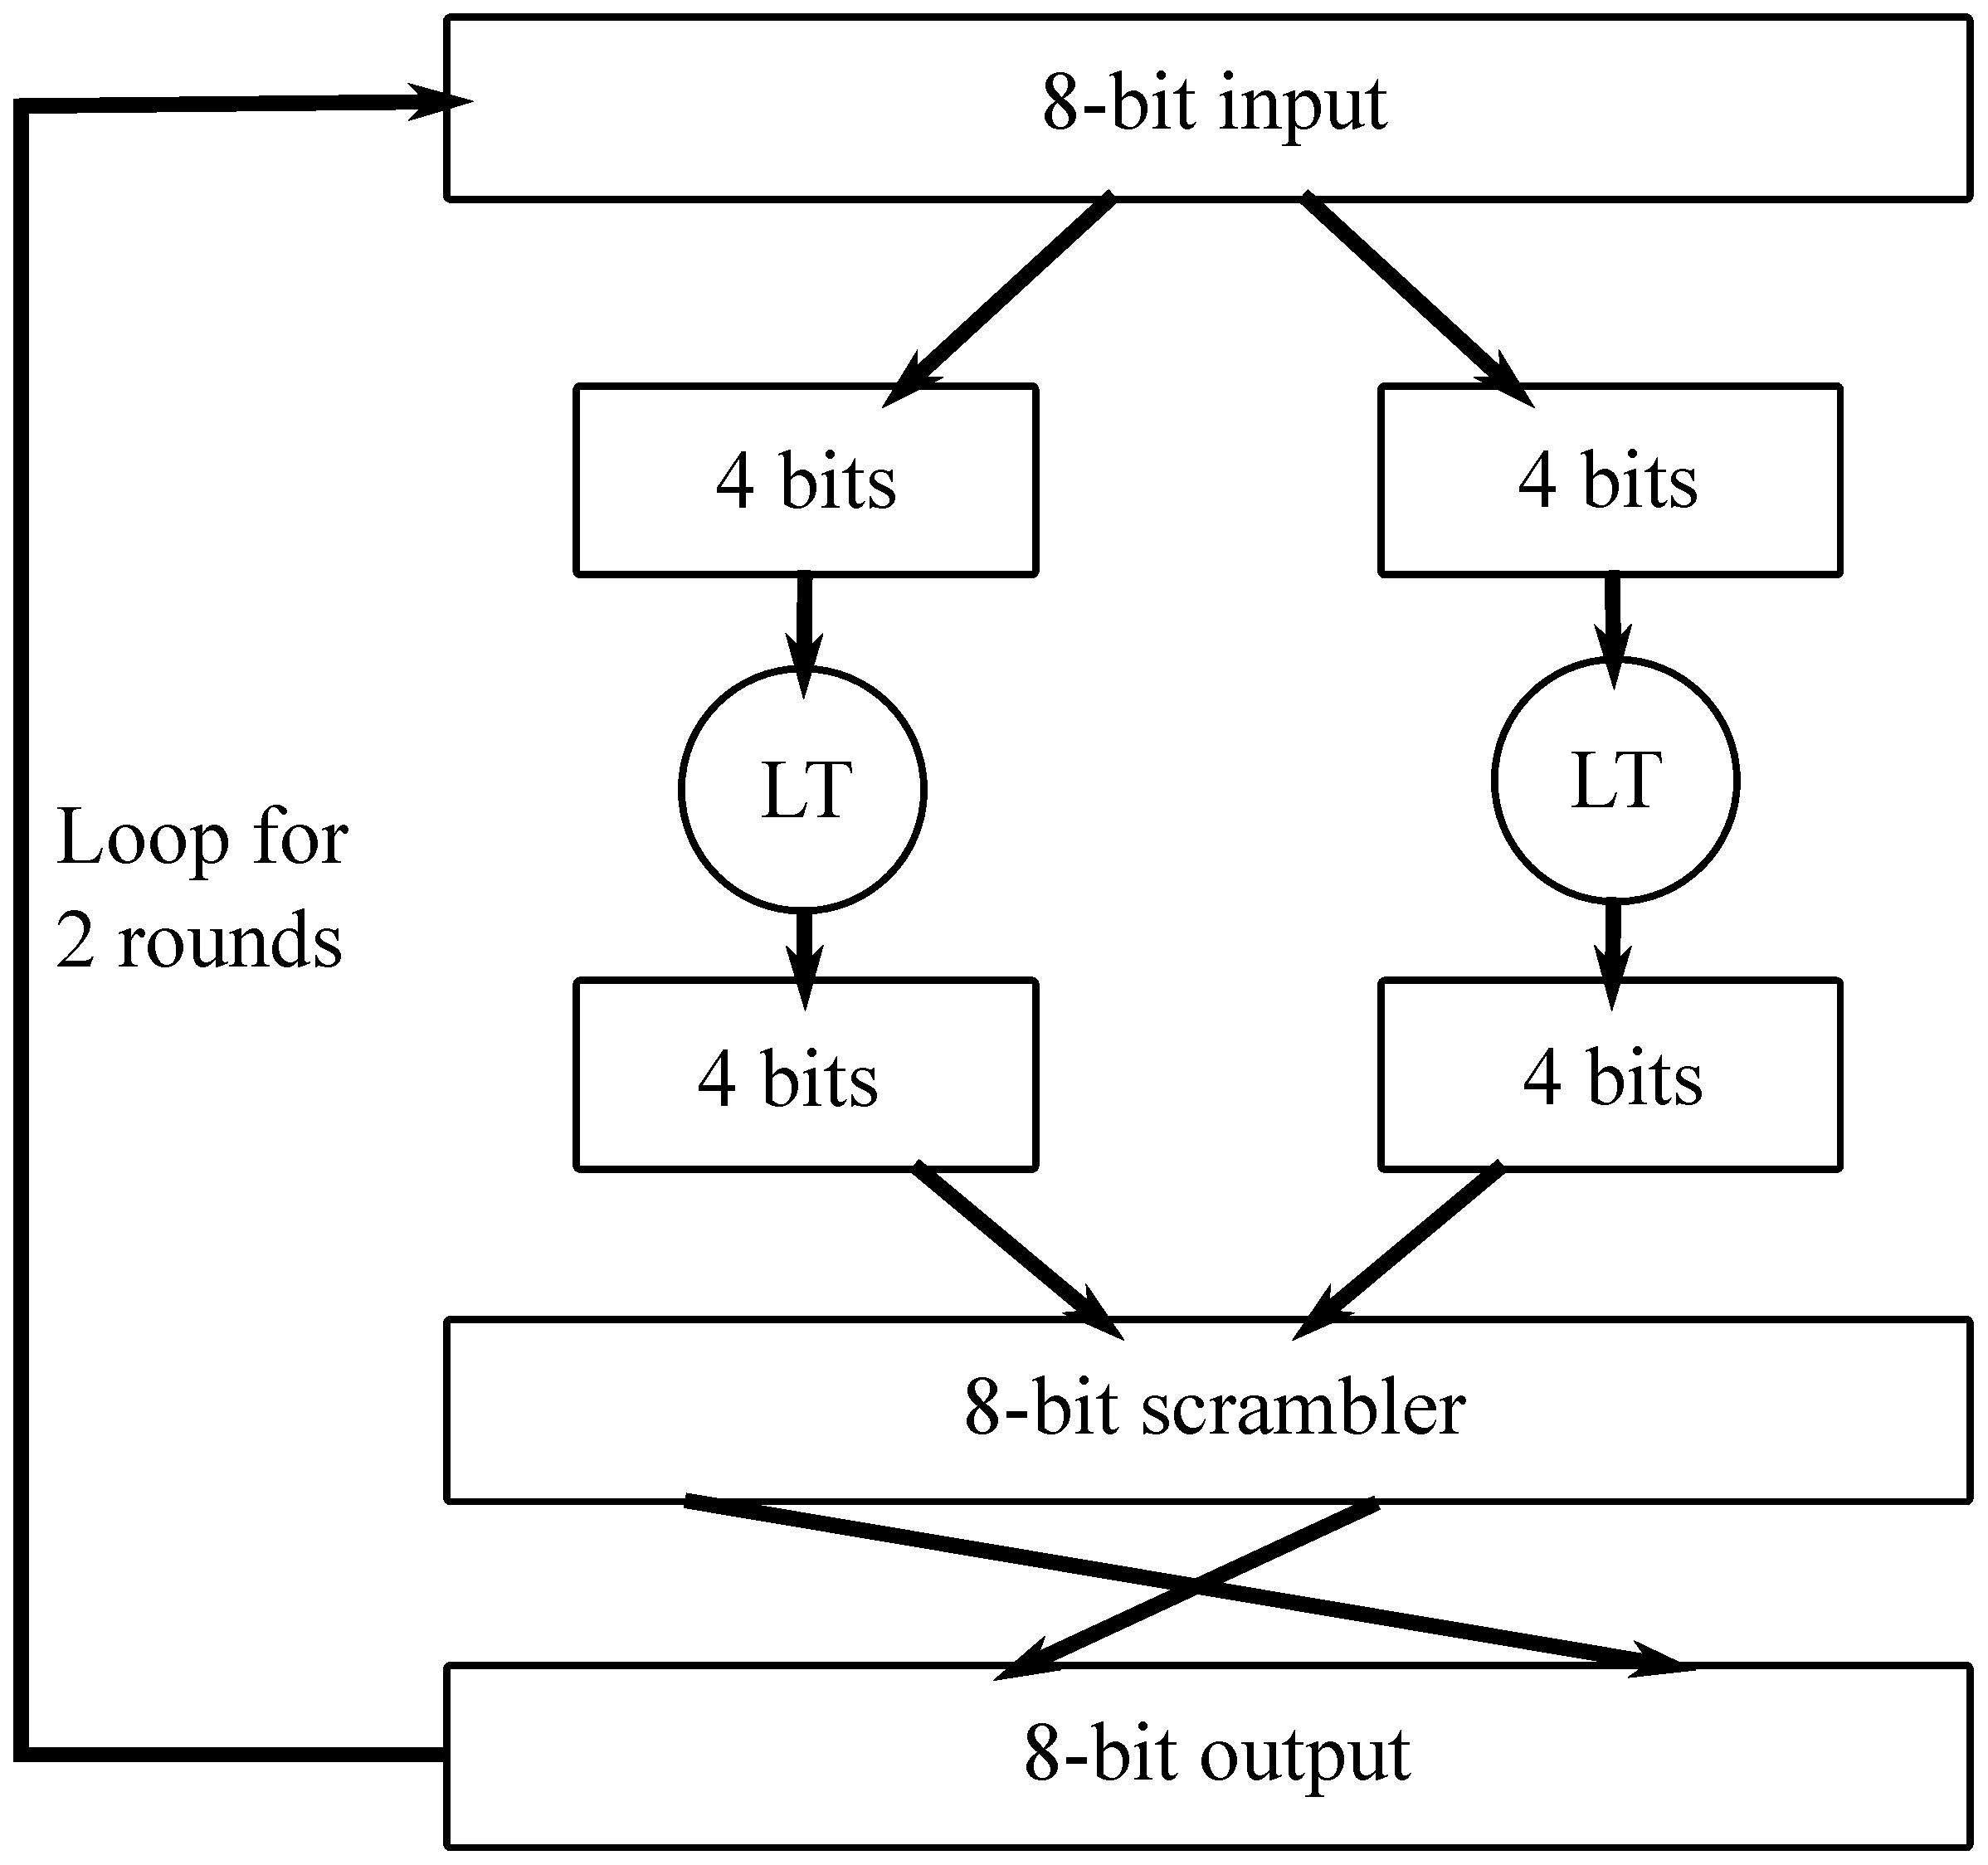
\includegraphics[width=80mm]{block_cipher.eps}
\end{figure}

(Hint: the LT circle blocks denote the look-up table of part a. You can refer to the descriptions of the figure 8.5 of the textbook for furthur explanations.)

Q4) Remember section 8.3 about message integrity. Assume our messages can only be 8-digit numbers (each digit can be 0 to 9) and a hash function takes such an 8-digit number and obtains a 10-digit number $a_0a_1a_2\cdots a_9$ where $$a_i=\text{number of }i\text{s in the input}$$
(e.g. 54756473 is mapped to 0001221200). If the 8-digit plain text is $33543612$, what is the probability that an intruder compromises the message having its hash output?

Q5) 

\begin{enumerate}[label=\alph*-]
\item
Recall the discussion about RSA (page 684, Public Key Encryption). Assume Alice encrypts her message by a public key $(77,13)$ and Bob and Jake each use a private key of $(77,37)$ and $(77,97)$ for decryption, respectively. Show that if Alice encrypts the number $2$ and sends it on the channel, then both Bob and Jake can decrypt it uniquely by calculating the details of RSA.
\item
(Extra Mark) Show that condition 3 in page 685 is necessary for condition $4$ (i.e. $4\implies 3$).
\end{enumerate}

Q6)

In the following encryption process, assume the circle blocks of + sign mean string concatenation. Also suppose that $K_A^+$, $K_A^-$, $K_B^+$, $K_B^-$ denote Alice's public and private key and Bob's public and private key. Also the Hash function block is denoted by $H(\cdot)$. Assume Alice generates a random key $S$ for using in both the Hash function and string concatenation (as indicated in the figure), before sending messages to Bob.
\begin{figure}[htbp]
\centering
\includegraphics[width=110mm]{q6_1.pdf}
\end{figure}
\begin{enumerate}[label=\alph*-]
\item
Sketch the necessary block diagram of message decryption at receiver (Bob's side).
\item
Which of confidentiality, end-to-end authentication and message integrity have not been preserved?
\item
Make as minimal as possible changes in the sender's (Alice's) encryption block diagram to fulfil the options of part b that were not preserved.
\end{enumerate}
\end{document}